\documentclass{article}
%
%\author{\\ \\ Carolyn McGraw \\ \\ Nuclear Engineering Department \\ \\}
%
\date{\today}
%
\title{\Huge{A Transport Sweep MiniApp:} \\ {\Large Documentaion and User Manual}}
%

%
%  mydefs.tex   
%  Command definitions that can be used in all documents that have
%      %
%  mydefs.tex   
%  Command definitions that can be used in all documents that have
%      %
%  mydefs.tex   
%  Command definitions that can be used in all documents that have
%      \input{mydefs}
%

%Load the myriad packages
%\usepackage{amssymb,amsmath}
\usepackage{amsfonts}
\usepackage{amsmath}
\usepackage{textcomp}
%\usepackage{graphicx}
\usepackage{grffile}
\usepackage{tikz}
%\usepackage{subeqn} %for eqn 1a, 1b, etc
\usepackage{subfig}    % for multi-figure figures
%\usepackage[numbers, super]{natbib}
%\usepackage{pdflscape}
%\usepackage{rotating}
%\usepackage{grffile} %spaces in file names
%\usepackage{parskip}
%\usepackage[T1]{fontenc} %for sc and bf
%\usepackage{wasysym}
%\usepackage{bigstrut}
%\usepackage{hyperref}
%\usepackage{Float}
\usepackage{multirow}
\usepackage[numbers,sort&compress]{natbib}

%Tikz libraries
\usetikzlibrary{calc,trees,positioning,arrows,chains,shapes.geometric,%
    decorations.pathreplacing,decorations.pathmorphing,shapes,%
    matrix,shapes.symbols}

% Optional for code samples
\usepackage{listings}
\lstloadlanguages{Matlab}
\lstset{language=Matlab,commentstyle=\color{blue},keywordstyle=\color{red}}

%MCNP syntax highlighting
\definecolor{lightgrey}{rgb}{0.9,0.9,0.9}
\definecolor{darkgreen}{rgb}{0,0.6,0}
 
\lstdefinelanguage{MCNP}
{morekeywords={kcode,ksrc,mode,print,prdmp},
sensitive=false,
morecomment=[f]{c},
morecomment=[l]{$},
morestring=[b]",
numbers=left,
numberstyle =\tiny,
}

\lstset{
language=Matlab,
numbers=left,
numberstyle =\tiny,}

%placeholder cite
\newcommand{\CITE}{({\bf cite})}
%singular
\newcommand{\fref}[1]{Fig.~\ref{fig:#1}}
\newcommand{\Fref}[1]{Figure~\ref{fig:#1}}
\newcommand{\eref}[1]{Eq.~(\ref{eq:#1})}
\newcommand{\Eref}[1]{Equation~(\ref{eq:#1})}
\newcommand{\tref}[1]{Table~\ref{tab:#1}}
%plural
\newcommand{\frefs}[2]{Figs.~\ref{fig:#1} and \ref{fig:#2}}
\newcommand{\Frefs}[2]{Figures~\ref{fig:#1} and \ref{fig:#2}}
\newcommand{\erefs}[2]{Eqs.~(\ref{eq:#1}) and (\ref{eq:#2})}
\newcommand{\Erefs}[2]{Equations~(\ref{eq:#1}) and (\ref{eq:#2})}
\newcommand{\trefs}[2]{Tables~\ref{tab:#1} and \ref{tab:#2}}
%range
\newcommand{\frefss}[2]{Figs.~\ref{fig:#1} - \ref{fig:#2}}
\newcommand{\Frefss}[2]{Figures~\ref{fig:#1} - \ref{fig:#2}}
\newcommand{\erefss}[2]{Eqs.~(\ref{eq:#1}) - (\ref{eq:#2})}
\newcommand{\Erefss}[2]{Equations~(\ref{eq:#1}) - (\ref{eq:#2})}
\newcommand{\trefss}[2]{Tables~\ref{tab:#1} - \ref{tab:#2}}
%misc.
\newcommand{\nn}[1]{\ensuremath{^{#1}}} %[1] is # of commands
\newcommand{\keff}{\ensuremath{{k_\mathrm{eff}}}}
\newcommand{\kinf}{\ensuremath{{k_\infty}}}
\newcommand{\alphaT}{\ensuremath{{\alpha_{_T}}}}
\newcommand{\SN}{\ensuremath{{\text{S}_n}}}
\newcommand{\PN}{\ensuremath{{\text{P}_n}}}
\newcommand{\order}[1]{\ensuremath{\mathcal{O}\left(#1\right)}}
% some simplifying commands
\newcommand{\eg}{e.g.}
%\newcommand{\eg}{{\it e.g.}} 
\newcommand{\ie}{i.e.}
\newcommand{\etal}{et al.}
\newcommand{\viz}{viz.}
\newcommand{\cf}{cf.}
\newcommand{\acite}[1]{{\bf(Add Citation: #1)}}
\newcommand{\E}{\mathcal{E}}
% derivative - d
\newcommand{\ud}[1]{\,\mathrm{d}{#1}\;}
% bold unit vector n-hat
\newcommand{\nhat}{\hat{\bf n}}
\newcommand{\tensor}[1]{\mathcal{#1}}
\renewcommand{\vec}[1]{\mathbf{#1}}
%Use for vectors of symbols (or use \pmb)
\newcommand{\vecsym}[1]{\boldsymbol{#1}}
\newcommand{\om}{\boldsymbol{\Omega}}

\newlength \figwidth
\setlength \figwidth {0.8\textwidth}
\captionsetup[subfigure]{width=0.4\textwidth} %trouble-maker
\captionsetup[subfigure]{font={footnotesize,stretch=1.1},skip=0pt}

 
 %LaTeX hyphenation
 \hyphenation{epi-thermal}

%Tikz flowchart parameters

\tikzstyle{block} = [rectangle, draw, fill=white, 
    text width=6em, text centered, rounded corners, minimum height=3em]
\tikzstyle{line} = [draw, thick, -latex']
 \tikzstyle{data} = [text width = 5em, text centered, node distance=1.6cm, inner sep=5pt] 
%

%Load the myriad packages
%\usepackage{amssymb,amsmath}
\usepackage{amsfonts}
\usepackage{amsmath}
\usepackage{textcomp}
%\usepackage{graphicx}
\usepackage{grffile}
\usepackage{tikz}
%\usepackage{subeqn} %for eqn 1a, 1b, etc
\usepackage{subfig}    % for multi-figure figures
%\usepackage[numbers, super]{natbib}
%\usepackage{pdflscape}
%\usepackage{rotating}
%\usepackage{grffile} %spaces in file names
%\usepackage{parskip}
%\usepackage[T1]{fontenc} %for sc and bf
%\usepackage{wasysym}
%\usepackage{bigstrut}
%\usepackage{hyperref}
%\usepackage{Float}
\usepackage{multirow}
\usepackage[numbers,sort&compress]{natbib}

%Tikz libraries
\usetikzlibrary{calc,trees,positioning,arrows,chains,shapes.geometric,%
    decorations.pathreplacing,decorations.pathmorphing,shapes,%
    matrix,shapes.symbols}

% Optional for code samples
\usepackage{listings}
\lstloadlanguages{Matlab}
\lstset{language=Matlab,commentstyle=\color{blue},keywordstyle=\color{red}}

%MCNP syntax highlighting
\definecolor{lightgrey}{rgb}{0.9,0.9,0.9}
\definecolor{darkgreen}{rgb}{0,0.6,0}
 
\lstdefinelanguage{MCNP}
{morekeywords={kcode,ksrc,mode,print,prdmp},
sensitive=false,
morecomment=[f]{c},
morecomment=[l]{$},
morestring=[b]",
numbers=left,
numberstyle =\tiny,
}

\lstset{
language=Matlab,
numbers=left,
numberstyle =\tiny,}

%placeholder cite
\newcommand{\CITE}{({\bf cite})}
%singular
\newcommand{\fref}[1]{Fig.~\ref{fig:#1}}
\newcommand{\Fref}[1]{Figure~\ref{fig:#1}}
\newcommand{\eref}[1]{Eq.~(\ref{eq:#1})}
\newcommand{\Eref}[1]{Equation~(\ref{eq:#1})}
\newcommand{\tref}[1]{Table~\ref{tab:#1}}
%plural
\newcommand{\frefs}[2]{Figs.~\ref{fig:#1} and \ref{fig:#2}}
\newcommand{\Frefs}[2]{Figures~\ref{fig:#1} and \ref{fig:#2}}
\newcommand{\erefs}[2]{Eqs.~(\ref{eq:#1}) and (\ref{eq:#2})}
\newcommand{\Erefs}[2]{Equations~(\ref{eq:#1}) and (\ref{eq:#2})}
\newcommand{\trefs}[2]{Tables~\ref{tab:#1} and \ref{tab:#2}}
%range
\newcommand{\frefss}[2]{Figs.~\ref{fig:#1} - \ref{fig:#2}}
\newcommand{\Frefss}[2]{Figures~\ref{fig:#1} - \ref{fig:#2}}
\newcommand{\erefss}[2]{Eqs.~(\ref{eq:#1}) - (\ref{eq:#2})}
\newcommand{\Erefss}[2]{Equations~(\ref{eq:#1}) - (\ref{eq:#2})}
\newcommand{\trefss}[2]{Tables~\ref{tab:#1} - \ref{tab:#2}}
%misc.
\newcommand{\nn}[1]{\ensuremath{^{#1}}} %[1] is # of commands
\newcommand{\keff}{\ensuremath{{k_\mathrm{eff}}}}
\newcommand{\kinf}{\ensuremath{{k_\infty}}}
\newcommand{\alphaT}{\ensuremath{{\alpha_{_T}}}}
\newcommand{\SN}{\ensuremath{{\text{S}_n}}}
\newcommand{\PN}{\ensuremath{{\text{P}_n}}}
\newcommand{\order}[1]{\ensuremath{\mathcal{O}\left(#1\right)}}
% some simplifying commands
\newcommand{\eg}{e.g.}
%\newcommand{\eg}{{\it e.g.}} 
\newcommand{\ie}{i.e.}
\newcommand{\etal}{et al.}
\newcommand{\viz}{viz.}
\newcommand{\cf}{cf.}
\newcommand{\acite}[1]{{\bf(Add Citation: #1)}}
\newcommand{\E}{\mathcal{E}}
% derivative - d
\newcommand{\ud}[1]{\,\mathrm{d}{#1}\;}
% bold unit vector n-hat
\newcommand{\nhat}{\hat{\bf n}}
\newcommand{\tensor}[1]{\mathcal{#1}}
\renewcommand{\vec}[1]{\mathbf{#1}}
%Use for vectors of symbols (or use \pmb)
\newcommand{\vecsym}[1]{\boldsymbol{#1}}
\newcommand{\om}{\boldsymbol{\Omega}}

\newlength \figwidth
\setlength \figwidth {0.8\textwidth}
\captionsetup[subfigure]{width=0.4\textwidth} %trouble-maker
\captionsetup[subfigure]{font={footnotesize,stretch=1.1},skip=0pt}

 
 %LaTeX hyphenation
 \hyphenation{epi-thermal}

%Tikz flowchart parameters

\tikzstyle{block} = [rectangle, draw, fill=white, 
    text width=6em, text centered, rounded corners, minimum height=3em]
\tikzstyle{line} = [draw, thick, -latex']
 \tikzstyle{data} = [text width = 5em, text centered, node distance=1.6cm, inner sep=5pt] 
%

%Load the myriad packages
%\usepackage{amssymb,amsmath}
\usepackage{amsfonts}
\usepackage{amsmath}
\usepackage{textcomp}
%\usepackage{graphicx}
\usepackage{grffile}
\usepackage{tikz}
%\usepackage{subeqn} %for eqn 1a, 1b, etc
\usepackage{subfig}    % for multi-figure figures
%\usepackage[numbers, super]{natbib}
%\usepackage{pdflscape}
%\usepackage{rotating}
%\usepackage{grffile} %spaces in file names
%\usepackage{parskip}
%\usepackage[T1]{fontenc} %for sc and bf
%\usepackage{wasysym}
%\usepackage{bigstrut}
%\usepackage{hyperref}
%\usepackage{Float}
\usepackage{multirow}
\usepackage[numbers,sort&compress]{natbib}

%Tikz libraries
\usetikzlibrary{calc,trees,positioning,arrows,chains,shapes.geometric,%
    decorations.pathreplacing,decorations.pathmorphing,shapes,%
    matrix,shapes.symbols}

% Optional for code samples
\usepackage{listings}
\lstloadlanguages{Matlab}
\lstset{language=Matlab,commentstyle=\color{blue},keywordstyle=\color{red}}

%MCNP syntax highlighting
\definecolor{lightgrey}{rgb}{0.9,0.9,0.9}
\definecolor{darkgreen}{rgb}{0,0.6,0}
 
\lstdefinelanguage{MCNP}
{morekeywords={kcode,ksrc,mode,print,prdmp},
sensitive=false,
morecomment=[f]{c},
morecomment=[l]{$},
morestring=[b]",
numbers=left,
numberstyle =\tiny,
}

\lstset{
language=Matlab,
numbers=left,
numberstyle =\tiny,}

%placeholder cite
\newcommand{\CITE}{({\bf cite})}
%singular
\newcommand{\fref}[1]{Fig.~\ref{fig:#1}}
\newcommand{\Fref}[1]{Figure~\ref{fig:#1}}
\newcommand{\eref}[1]{Eq.~(\ref{eq:#1})}
\newcommand{\Eref}[1]{Equation~(\ref{eq:#1})}
\newcommand{\tref}[1]{Table~\ref{tab:#1}}
%plural
\newcommand{\frefs}[2]{Figs.~\ref{fig:#1} and \ref{fig:#2}}
\newcommand{\Frefs}[2]{Figures~\ref{fig:#1} and \ref{fig:#2}}
\newcommand{\erefs}[2]{Eqs.~(\ref{eq:#1}) and (\ref{eq:#2})}
\newcommand{\Erefs}[2]{Equations~(\ref{eq:#1}) and (\ref{eq:#2})}
\newcommand{\trefs}[2]{Tables~\ref{tab:#1} and \ref{tab:#2}}
%range
\newcommand{\frefss}[2]{Figs.~\ref{fig:#1} - \ref{fig:#2}}
\newcommand{\Frefss}[2]{Figures~\ref{fig:#1} - \ref{fig:#2}}
\newcommand{\erefss}[2]{Eqs.~(\ref{eq:#1}) - (\ref{eq:#2})}
\newcommand{\Erefss}[2]{Equations~(\ref{eq:#1}) - (\ref{eq:#2})}
\newcommand{\trefss}[2]{Tables~\ref{tab:#1} - \ref{tab:#2}}
%misc.
\newcommand{\nn}[1]{\ensuremath{^{#1}}} %[1] is # of commands
\newcommand{\keff}{\ensuremath{{k_\mathrm{eff}}}}
\newcommand{\kinf}{\ensuremath{{k_\infty}}}
\newcommand{\alphaT}{\ensuremath{{\alpha_{_T}}}}
\newcommand{\SN}{\ensuremath{{\text{S}_n}}}
\newcommand{\PN}{\ensuremath{{\text{P}_n}}}
\newcommand{\order}[1]{\ensuremath{\mathcal{O}\left(#1\right)}}
% some simplifying commands
\newcommand{\eg}{e.g.}
%\newcommand{\eg}{{\it e.g.}} 
\newcommand{\ie}{i.e.}
\newcommand{\etal}{et al.}
\newcommand{\viz}{viz.}
\newcommand{\cf}{cf.}
\newcommand{\acite}[1]{{\bf(Add Citation: #1)}}
\newcommand{\E}{\mathcal{E}}
% derivative - d
\newcommand{\ud}[1]{\,\mathrm{d}{#1}\;}
% bold unit vector n-hat
\newcommand{\nhat}{\hat{\bf n}}
\newcommand{\tensor}[1]{\mathcal{#1}}
\renewcommand{\vec}[1]{\mathbf{#1}}
%Use for vectors of symbols (or use \pmb)
\newcommand{\vecsym}[1]{\boldsymbol{#1}}
\newcommand{\om}{\boldsymbol{\Omega}}

\newlength \figwidth
\setlength \figwidth {0.8\textwidth}
\captionsetup[subfigure]{width=0.4\textwidth} %trouble-maker
\captionsetup[subfigure]{font={footnotesize,stretch=1.1},skip=0pt}

 
 %LaTeX hyphenation
 \hyphenation{epi-thermal}

%Tikz flowchart parameters

\tikzstyle{block} = [rectangle, draw, fill=white, 
    text width=6em, text centered, rounded corners, minimum height=3em]
\tikzstyle{line} = [draw, thick, -latex']
 \tikzstyle{data} = [text width = 5em, text centered, node distance=1.6cm, inner sep=5pt] 

%\linespread{1}
\addtolength{\hoffset}{-1.8cm}
\addtolength{\textwidth}{3.6cm}
\addtolength{\voffset}{-1.2cm}
\addtolength{\textheight}{2.4cm}
%
%Brian's package
\usepackage{fancyhdr}
\usepackage{tablefootnote}
\usepackage{float}
\usepackage{listings}
\pagestyle{fancy}
\fancyhf{}
\fancyhead{}
\lhead{McGraw, Adams}
\rhead{\rightmark}%\today}
\cfoot{\thepage}
%

\renewcommand{\ss}{ss}

\begin{document}

  \begin{titlepage}
    \vspace*{\fill}
    \begin{center}
      {\Huge{A Transport Sweep MiniApp:}}\\[0.5cm]
      {\huge {Users Manual}}\\[0.5cm]
    \end{center}
    \vspace*{\fill}
  \end{titlepage}

%%%%%%%%%%%%%%%%%%%%%%%%%%%%%%%%%%%%%%%%%%%%%%%%%%
%
\section{Introduction}
%
DFEComm is a mini-app developed for the Center for Exascale Simulation of Advanced Reactors (CESAR) co-design center. The mini-app is purposed with simulating the performance characteristics of software that utilizes transport sweeps to solve the neutron transport equation. \\

This user manual will briefly illustrate how parallel transport sweeps are performed, detail the input file format used in DFEComm, and describe the options available to the user. The Future Work section will outline features to be implemented in future versions of DFEComm.


%%%%%%%%%%%%%%%%%%%%%%%%%%%%%%%%%%%%%%%%%%%%%%%%%%
\section{Parallel Transport Sweeps}
The $S_N$, or discrete ordinates, form of the neutron transport equation is:
\begin{equation}
  \hat \Omega_m \cdot \nabla \psi_m^g ( \vec r )  + \sigma_t^g ( \vec r ) \psi_m^g ( \vec r) = q_{tot}^g(\vec r,\hat \Omega_m),
\label{eq::group_trans}
\end{equation}
where $\psi_m^g ( \vec r )$ is the angular flux, $\sigma_t^g ( \vec r )$ is the macroscopic total cross section, $ q_{tot}^g(\vec r,\hat \Omega_m)$ is the total neutron source, and $\hat \Omega_m$ is the $m^{th}$ quadrature direction. The total source provides the only coupling between quadrature directions. If the source is lagged, the equation for each angle can be solved independently of the others. A \emph{sweep} solves Eq. \ref{eq::group_trans} with a given iterate for the total source for all directions and energies. \\

Equation \ref{eq::group_trans} is solved in each spatial cell through an upwinding scheme in which information from cells \emph{upstream} of the current cell is used as a boundary condition. Here, \emph{upstream} is defined as in the direction opposite the current quadrature direction, and \emph{upstream cells} are those for which the solution has already been calculated. Once the equation is solved in the cell, the solution is then transmitted to its \emph{downstream} neighbor. In this way, the method \emph{sweeps} through the problem. \\

Take for example a 1D mesh, seen in Figure \ref{fig::1Dmesh}. Given a sweep direction in the positive x direction, cell 1 must be solved first, using information from the left boundary of the problem. Once the angular flux in cell 1 has been computed, cell 2 may be solved using the solution in cell 1. Then cell 3 can be computed using cell 2's solution, etc. For this sweep direction, cell 1 is considered upstream of cell 2, and cell 2 is downstream of cell 1. Likewise, if the sweep direction is in the negative x direction, cell 8 must be solved first using information from the right boundary, followed by 7, then 6, etc. In this case, cell 1 would be downstream of cell 2, and cell 2 would be upstream of cell 1.

\begin{figure}[ht!]
  \begin{center}
  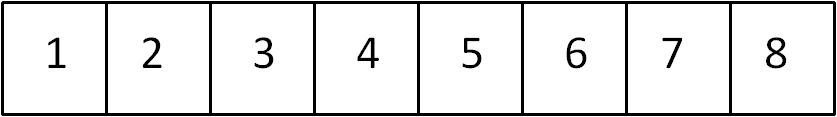
\includegraphics[width=0.7\textwidth]{Images/1D_sweep.png}
    \caption[]{1D mesh}\label{fig::1Dmesh}
  \end{center}
\end{figure}

When solving Eq. \ref{eq::group_trans} using multiple processes, the spatial mesh is \emph{partitioned} among the shared memory locations, or SMLs. A shared memory location is a unit of computational hardware which has a shared block of memory. For example, this could be a single MPI process, or a node with multiple threads. Details on the partitioning process are described below in Section \ref{sec::Partition}. Given a partitioning, the spatial cells, quadrature directions, and energy groups are \emph{aggregated} into cellsets, anglesets, and groupsets, respectively. A triplet of cellset, angleset, and groupset define a \emph{task}. A \emph{task} is then defined as the amount of work an SML must perform before communicating to its downstream neighbors. A simple, reasonably good model for parallel sweep efficiency is: 
\begin{equation} 
  		E \approx \frac{1}{\left[ 1 + \frac{N_{idle}}{N_{tasks}} \right] \left[ 1 + \frac{T_{comm}}{T_{task}} \right] } 
\end{equation}
where $N_{idle}$ is the number of idle stages each process has, $N_{tasks}$ is the number of tasks each SML performs, $T_{comm}$ is the communication time, and $T_{task}$ is the time it takes to perform a task. The aggregation of the problem allows the parallel efficiency to be optimized. For example, choose a large number of tasks minimizes the first bracketed term, but maximizes the second, since the time per task is approximately inversely proportional to the number of tasks.


%%%%%%%%%%%%%%%%%%%%%%%%%%%%%%%%%%%%%%%%%%%%%%%%%%
\section{Partitioning} \label{sec::Partition}
 In their 2009 presentation at the Mathematics, Computational Methods, and Reactor Physics conference, Bailey and Falgout presented a generalized method for partitioning the spatial mesh among multiple processes. The terminology in that paper is used in DFEComm, and is briefly described below. The reader is referred to \cite{BaileyFalgout}, \cite{sweep-trans}, and \cite{opt-sweep} for more detailed discussions on the theory behind and analysis of these partitioning methods as they are applied to transport sweeps. \\

Each dimension (in SML space) is given one of two \emph{distribution functions}: round robin or blocked. Round robin refers to a sequence that increments and then repeats, e.g. 1 2 3 4 1 2 3 4. Blocked refers to a sequence that repeats and then increments, e.g. 1 1 2 2 3 3 4 4. Each dimension is also given an \emph{overload factor}, which is the number of spatial cellsets given to each SML. In the previous examples, the overload factor is 2 (each number is repeated twice). Finally, each dimension is given a total number of spatial cellsets that the mesh is broken up into. In both previous examples, the number of cellsets is 8 (there are 8 numbers). The quotient of the total number of cellsets and the overload factor is the number of SMLs in that dimension. The total number of SMLs is the product of the number of SMLs in each dimension. \\
 
 In DFEComm, there are several preset partitioning schemes available to the user: Koch-Baker-Alcouffe (KBA), Hybrid-KBA, Volumetric, and Volumetric with Round Robin. In addition, the user is allowed to define their own partitioning scheme using partition functions, overload factors, and total number of cellsets. Table \ref{table::partition} defines the partitioning parameters for these pre-defined schemes. The implementation of these preset partitions are found in \emph{Problem\_Input.cc} in the \emph{GetPartitionParameters()} function, if the user would like to define their own. As a note, the division by 2 in the number of cellsets for partition types 0 and 2 are removed if the problem is run on 1 SML.\\

\begin{table}[H]
\begin{center}
  \begin{tabular}{ |c| p{4cm}| c| p{3cm}| p{3.0cm}|}
    \hline
    Partition &  & Partition & \multicolumn{1}{c|}{Overload} &\multicolumn{1}{c|}{ Number of } \\ 
    Type & \multicolumn{1}{c|}{Description} &  Function &  \multicolumn{1}{c|}{ Factor} &\multicolumn{1}{c|}{Cellsets (in x,y, and z) }\\ 
    \hline& & & &\\ [-1.5ex]
    0 & Default Hybrid-KBA & Blocked  & x = 1, & x = $\sqrt{\frac{\text{\# SML}}{2}}$  \\  
     &  && y = 1,  & y =$\sqrt{\frac{\text{\# SML}}{2}}$ \\  
     & & & z = \emph{z\_planes} &  z = $\frac{\emph{z\_planes}}{2}$\\
    \hline& & & &\\ [-1.5ex]
     1 & KBA & Blocked  & x = user defined & x = $\sqrt{\frac{\text{\# SML}}{\text{overload}}}$ \\  
     &   && y =  user defined  & y = $\sqrt{\frac{\text{\# SML}}{\text{overload}}}$ \\  
     & & & z = \emph{z\_planes} &  z = \emph{z\_planes}\\
     \hline& & & &\\ [-1.5ex]
    2 & Hybrid-KBA & Blocked  & x = user defined & x = $\sqrt{\frac{\text{\# SML}}{2*\text{overload}}}$  \\  
     &  && y = user defined  & y = $\sqrt{\frac{\text{\# SML}}{2*\text{overload}}}$ \\  
     & & & z = \emph{z\_planes} & z = $\frac{\emph{z\_planes}}{2}$\\
    \hline& & & &\\ [-1.5ex]
    4 & Volumetric & Blocked  & x = 1 & x = $\text{\# SML}^{1/3}$ \\  
     &  && y = 1  & y = $\text{\# SML}^{1/3}$ \\  
     & & & z = 1 & z = $\text{\# SML}^{1/3}$\\
    \hline& & & &\\ [-1.5ex]
    5 & Volumetric & Round Robin  & x = user defined & x =$\left(\frac{\text{\# SML}}{\text{overload}}\right)^{1/3}$ \\  
     & with Round Robin && y = user defined  & y = $\left(\frac{\text{\# SML}}{\text{overload}}\right)^{1/3}$ \\  
     & & & z = user defined & z =$\left(\frac{\text{\# SML}}{\text{overload}}\right)^{1/3}$\\
      \hline& & & &\\ [-1.5ex]
    6 & User Defined Partitioning &User Defined& \multicolumn{1}{l|}{x,y, z = user defined } & \multicolumn{1}{l|}{x,y, z = user defined }\\  
    \hline
  \end{tabular} 
  
      \caption{Partition Types}
      \label{table::partition}
\end{center}
\end{table}


 \subsection{Auto-partitioning}
Currently, DFEComm has the ability to auto-partition the mesh. Given an SML count, the code attempts to find the optimal layout of SMLs. The ideal case is a hybrid-KBA layout with 2 SMLs in the z dimension, and $\sqrt{\frac{\# \text{SML}}{2}}$ SMLs in both the x and y dimensions. If $\sqrt{\frac{\# \text{SML}}{2}}$ is not an integer, a function computes the prime factorization of $\sqrt{\frac{\# \text{SML}}{2}}$ and chooses an SML layout closest to a square, assigning the larger SML count to the x dimension. For example, given 12 SMLs, the auto-partition function would provide a layout of 4 SMLs in x, 3 in y, and 2 in z. An even number of SMLs is required so that the z-dimension can always be divided into 2 and that hybrid-KBA can be used. Currently auto-partitioning is available only for the preset problem sizes, defined in Section \ref{probdef}.

%%%%%%%%%%%%%%%%%%%%%%%%%%%%%%%%%%%%%%%%%%%%%%%%%%
\section{Compiling and Running DFEComm}
DFEComm is available for download on GitHub. To clone the repository on GitHub:
\begin{verbatim}
>$ git clone https://github.com/cnmcgraw/DFEComm.git
\end{verbatim}
Once cloned, the code can be updated to the newest version using the following command (when in the DFE\_Comm directory):
\begin{verbatim}
>$ git pull
\end{verbatim}
 DFEComm is built upon MPI and has been tested using mpi++ as its compiler. To compile DFEComm, use the following command:
\begin{verbatim}
>$ make
\end{verbatim}
To run DFEComm, use the following command:
\begin{verbatim}
>$ mpirun -n [# SML] ./DFEComm -f [Input file]
\end{verbatim}
Here the input file must be a text file in the format described in the next section. The number of SMLs indicated at run time must match that found in the input file.

%%%%%%%%%%%%%%%%%%%%%%%%%%%%%%%%%%%%%%%%%%%%%%%%%%
\section{Input File Structure}
The input file is a text file with a listing of case sensitive keywords separated from their values by an ``='' surrounded by at least one set of spaces. Lines beginning with ``\#'' followed by at least one space are comments. The file format can take multiple formats, and blank lines and the order of keywords do not matter. A listing of all available keywords, their definitions, and their available values is seen in Table \ref{table::parameters}.  Several example inputs are available with the DFEComm source code to assist users. \\

\begin{table}[h!]
\begin{center}
  \begin{tabular}{ |c|p{5cm}|c|p{6.4cm}|}
    \hline
    Input &\multicolumn{1}{c|}{ Values} &  Default& \\ 
    Parameter & \multicolumn{1}{c|}{Allowed}&Value& \multicolumn{1}{c|}{Definition}\\
    \hline
    problem\_size & 0,1,2,3,4 & 0& Predefined Problem Size per SML\\  \hline
    num\_pin\_x& Positive Integer & None &  Number of fuel pins in the x-dimension\\ 
    num\_pin\_y& Positive Integer & None &  Number of fuel pins in the y-dimension\\
    refinement & Positive Integer & None & Number of `rings' in each fuel pin \\
    z\_planes& Positive Integer & None &  Number of mesh cells in the z-dimension\\ 
    bc & 1,2 & 2 & Boundary Conditions, 1 = Reflecting, 2 = Incident Flux \\ \hline
    num\_polar & Positive Even Integers& None &  Total number of polar angles \\
    num\_azim & Positve Integers Divisible by 4&  None& Total number of azimuthal angles \\
    angle\_aggregation & 1,2,3 & None & Angle Aggregation, 1 = Single, 2 = Polar, 3 = Octant \\ \hline
    num\_groups & Positive Integer, Divisible by num\_groupsets & None & Total number of energy groups \\ 
    num\_groupsets & Positive Integer & None & Number of energy groupsets \\ \hline
    num\_SML & Positive Integer & None & Number of Shared Memory Locations \\
    partition\_type & 0,1,2,3,4,5,6 & 0 & Type of spatial partitioning, options explained in Table \ref{table::partition} \\
    func\_\{x,y,z\} & 1,2 & None & Partition function to use in \{x,y,z\}, 1 = blocked, 2 = round robin \\
    overload\_\{x,y,z\} & Positive Integer & None & Overload factor in \{x,y,z\} \\
    overload & Positive Integer & None & Total overload factor, used with partition\_type = 1,2, and 4 \\
    num\_cellsets\_\{x,y,z\} & Positive Integer & None & Total number of cellsets to divide the problem into in \{x,y,z\} \\ 
    num\_sweeps & Positive Integer & None & Number of transport sweeps to perform and average over \\
    \hline
  \end{tabular} 
      \caption{All Available Input Parameters}
      \label{table::parameters}
\end{center}
\end{table}

An example of the most verbose form of the input file can be seen in Figure \ref{fig::verbose}. This form allows the user complete control over the definition of their problem. This example defines a problem with 2 cellsets, each with a 16x16x16 mesh layout. Each of the two SMLs specified have one cellset. There are 80 total angles, and octant aggregation is used. There is one groupset, with one energy group. Finally, 10 sweeps will be performed and the average time per sweep will be reported. This example is found in \emph{Example\_Input.txt} in the DFEComm folder.\\
\begin{figure}[H]
\begin{verbatim}
# Space
num_pin_x = 1
num_pin_y = 1
refinement = 8
z_planes = 32
bc = 2

# Angle
num_polar = 10
num_azim = 8
angle_aggregation = 3

# Energy
num_groups = 1
num_groupsets = 1
  	
# Partitioning
num_SML = 2
partition_type = 6
  	
func_x = 1
overload_x = 1
num_cellsets_x = 1
func_y = 1
overload_y = 1
num_cellsets_y = 1
func_z = 1
overload_z = 1
num_cellsets_z = 2

num_sweeps = 10
\end{verbatim}
  \caption[]{Example Verbose Input File}\label{fig::verbose}
\end{figure}

On the other end the spectrum, a much simpler form of the input can be seen in Figure \ref{fig::simplified}. This form is intended to allow the user to define a problem using the least amount of keywords. DFEComm has as a collection of preset problems which are defined per SML, specified with only one keyword, \emph{problem\_size}. The specifics of these predefined problems are detailed in the next section. For this input format, only the number of SMLs and the number of sweeps to perform are further required. DFEComm uses the auto-partitioning function and hybrid-KBA to divide the mesh among the SMLs. This example input is found in \emph{Example\_Input\_ProblemSize.txt} in the DFEComm folder.\\

\begin{figure}[H]
\begin{verbatim}
# Simplified Input
problem_size = 1
num_SML = 2
num_sweeps = 5
\end{verbatim}  
    \caption[]{Example Simplified Input File}\label{fig::simplified}
\end{figure}

An example of an input using one of the predefined partitioning schemes in seen in Figure \ref{fig::partition}. The \emph{overload} keyword, required for \emph{partition\_types} 1, 2, and 4, defines the overload factor for both the x and y dimensions. \\

\begin{figure}[htbp]
\begin{verbatim}
# Space
num_pin_x = 1
num_pin_y = 1
refinement = 8
z_planes = 32
bc = 2

# Angle
num_polar = 10
num_azim = 8
angle_aggregation = 3

# Energy
num_groups = 1
num_groupsets = 1
  	
# Partitioning
num_SML = 2
partition_type = 2	
overload = 1

num_sweeps = 10
 \end{verbatim}  
    \caption[]{Example Predefined Partitioning Input File}\label{fig::partition}
\end{figure}

%%%%%%%%%%%%%%%%%%%%%%%%%%%%%%%%%%%%%%%%%%%%%%%%%%
\subsection{Pre-defined Problems} \label{probdef}
Four predefined problems are available in DFEComm to enable weak scaling studies. Each problem size, defined in Table \ref{table::probsize}, is defined per SML. The angular quadrature is aggregated by octant, and the energy groups are aggregated into one groupset. Currently, the spatial mesh is aggregated into one cellset per SML. This will be optimized in future versions of DFEComm. The largest of these problems (4), is intended to test the limits of the machine DFEComm is run on. It is also meant to be extended to an on-node mini-app in which the quadrature and energy groups are split up over threads on a SML.\\ \newline

\begin{table}[H]
\begin{center}
  \begin{tabular}{ |c| c | c|c| c|}
    \hline
    Problem & Spatial & Quadrature& Number of & Unknowns per \\ 
    Size ID & Mesh& (\# Polar $\times$ \# Azimuthal) &  Energy Groups & Task per SML\\
    \hline
    1 & 2 x 2 x 10 & 4 x 4 & 10 & 800\\ 
    2 & 10 x 10 x 100 & 4 x 16 & 50& 4M\\
    3 & 10 x 10 x 200& 16 x 16 & 100& 64M \\
    4 & 10 x 10 x 200& 16 x 64 & 500 & 1.2B \\
    \hline
  \end{tabular} 
      \caption{Pre-defined Problem Definitions}
      \label{table::probsize}
\end{center}
\end{table}


%%%%%%%%%%%%%%%%%%%%%%%%%%%%%%%%%%%%%%%%%%%%%%%%%%
\subsection{Future Work} \label{future}
DFEComm is an ongoing research effort, and therefore is still under active development. As such, a few desired features not yet implemented into DFEComm are set to become available soon. This includes:
\begin{itemize}
	\item Reflecting Boundary Conditions
	\item Allowing the number of SMLs to be defined via the command line
	\item Defining a default number of sweeps to perform
	\item Multiple Cellsets per SML
	\item Optimization of data movement to improve weak scaling efficiency
\end{itemize}

%%%%%%%%%%%%%%%%%%%%%%%%%%%%%%%%%%%%%%%%%%%%%%%%%%
%
\pagebreak
\bibliographystyle{elsart-num-names}
\renewcommand{\bibname}{{\normalsize\rm REFERENCES}}
%\nocite{*}
\begin{thebibliography}{300}
\bibitem{BaileyFalgout} T.\ S.\ Bailey and R.\ D.\ Falgout, ``Analysis Of Massively Parallel Discrete-Ordinates Transport Sweep Algorithms With Collisions," {\em Proc. International Conference on Mathematics, Computational Methods \& Reactor Physics}, Saratoga Springs, May 3-7, CDROM (2009).

\bibitem{sweep-trans} W. Daryl Hawkins, Timmie Smith, Michael P. Adams, Lawrence Rauchwerger, Nancy M. Amato, and Marvin L. Adams, ``Efficient Massively Parallel Transport Sweeps," {\it Trans. Amer. Nucl. Soc.}, {\bf 107}, pp.\ 477-481 (2012).

\bibitem{opt-sweep} M.P. Adams, M.L. Adams, W.D. Hawkins, T. Smith, L. Rauchwerger, N.M. Amato, T.S. Bailey, R.D. Falgout, ``Provably Optimal Parallel Transport Sweeps On Regular Grids," {\em Proc. International Conference on Mathematics and Computational Methods applied to Nuclear Science and Engineering}, Sun Valley, Idaho, USA, May 5-9, CD-ROM (2013).


\end{thebibliography}


\end{document}


%\begin{figure}[ht!]
%  \begin{center}
%  \includegraphics[width=1\textwidth]{Images/3D_full_layout.jpg}
%    \caption[]{Top-Down and Two Side Layouts of the 3D C5G7 Benchmark Problem}\label{fig::3Dlayout}
%  \end{center}
%\end{figure}
